\documentclass[12pt, letterpaper]{article}
\usepackage{graphicx}
\usepackage[margin=1in]{geometry}
\usepackage{amsmath, amssymb, amsthm, mathrsfs}
\usepackage{fancyhdr}
\usepackage{tikz}
\usepackage{enumerate}
\usepackage{cancel}
\usetikzlibrary{positioning}
\usepackage[utf8]{inputenc}
\usepackage{xcolor}
\usepackage{framed}
\title{HW 1.3}
\author{Your Name}
\date{\today}
\pagestyle{fancy}
\renewcommand{\headrulewidth}{0pt}
\renewcommand{\footrulewidth}{0pt}
\fancyhf{}
\rhead{
    Zack Abdirashid\\
    2/12/26 \\
    MATH 405
}
\rfoot{Page \thepage}
\begin{document}
\paragraph{\underline{1.4} \\ \\} 
\textbf{7.} In each case, give the values of $\textbf{r, e,}$ or $\textbf{v}$ (whichever is not given) assuming that the graph is planar. Then either draw a connected, planar graph with the property, if possible, or explain why no such planar graph can exist. \\ \\
\indent \textbf{(d)} $14$ edges and nine regions
\begin{center}
    $r = 9$, $e = 14$, $v$ = ? 
\end{center}
\begin{align*}
     * \ &r = e - v + 2 \\
    \Rightarrow \ &9 = 14 - v + 2 \\
    \Rightarrow \ &-7 = -v \\
    \Rightarrow \ &\boxed{v = 7} \\ \\
    * \ &e \leq 3v - 6 \\
    \Rightarrow \ &14 \leq 3(7) - 6 = 15 \ \checkmark
\end{align*}
\begin{center}
    \begin{tikzpicture}[scale=1.5, every node/.style={circle, fill=black, inner sep=1.5pt}]

    % Define the 7 Vertices (Matching the layout of the screenshot)
    \node[label=above left:1] (V1) at (0, 1.5) {};
    \node[label=above:2]      (V2) at (1.5, 1.5) {};
    \node[label=above:3]      (V3) at (3, 1.5) {};
    \node[label=below:4]      (V4) at (0, 0) {};
    \node[label=below:5]      (V5) at (0.8, 0) {};
    \node[label=below:6]      (V6) at (2.2, 0) {};
    \node[label=below:7]      (V7) at (3, 0) {};

    % Draw the Edges (Lines and Curves)
    \begin{scope}[thick]
        % Horizontal and Vertical straight lines
        \draw (V1) -- (V2) -- (V3); % Top edge
        \draw (V4) -- (V5) -- (V6) -- (V7); % Bottom edge
        \draw (V1) -- (V4); % Left edge
        \draw (V3) -- (V7); % Right edge
        
        % Diagonal lines (The zig-zag inside)
        \draw (V1) -- (V5);
        \draw (V5) -- (V2);
        \draw (V2) -- (V6);
        \draw (V6) -- (V3);

        % Curved lines for external regions
        % Region 6: Loop from 1 to 5
        \draw (V1) to[out=185, in=225, looseness=3] (V5); 
        
        % Region 7: Loop from 2 to 7
        \draw (V2) to[out=50, in=55, looseness=2.5] (V7);
        
        % Region 8: Large outer loop from 1 to 7
        \draw (V1) to[out=55, in=40, looseness=3] (V7);
    \end{scope}

    % Region Labels (Face numbers)
    \begin{scope}
        \node[fill=none] at (0.3, 0.5)  {A};
        \node[fill=none] at (0.8, 1.0)  {B};
        \node[fill=none] at (1.5, 0.5)  {C};
        \node[fill=none] at (2.2, 1.0)  {D};
        \node[fill=none] at (2.7, 0.5)  {E};
        
        % Outer Region Labels
        \node[fill=none] at (-0.4, 0.5) {F};
        \node[fill=none] at (3.2, 1.1)  {G};
        \node[fill=none] at (2.8, 2.7)  {H};
        \node[fill=none] at (4.5, 1.5)  {I};
    \end{scope}
\end{tikzpicture}
\end{center}
\hspace{0.3em}
\textbf{(f)} Five regions and 10 edges 
\begin{center}
     $r = 5$, $e = 10$, $v = $?
\end{center}
\begin{align*}
    * \ &r = e - v + 2 \\
    \Rightarrow \ &5 = 10 - v + 2 \\
    \Rightarrow \ &-7 = -v \\
    \Rightarrow \ &\boxed{v = 7} \\ \\
    * \ &e \leq 3v - 6 \\
    \Rightarrow \ & 10 \leq 3(7) - 6 = 15 \ \checkmark
\end{align*}
\begin{center} 
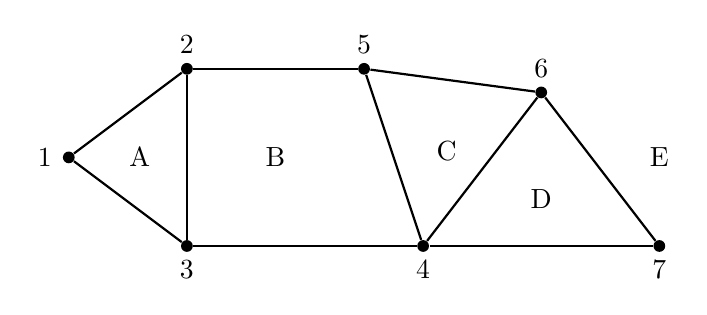
\begin{tikzpicture}[scale=1.5, every node/.style={circle, fill=black, inner sep=1.5pt}]
    % Define the 7 Vertices (a-g)
    \node[label=above:2] (a) at (1, 2) {};
    \node[label=above:5] (b) at (2.5, 2) {};
    \node[label=above:6] (c) at (4, 1.8) {};
    \node[label=below:4] (d) at (3, 0.5) {};
    \node[label=below:3] (e) at (1, 0.5) {};
    \node[label=below:7] (f) at (5, 0.5) {};
    \node[label=left:1] (g) at (0, 1.25) {};

    % Draw the Edges (Straight Lines)
    \begin{scope}[thick]
        % Outer boundary and internal dividers
        \draw (g) -- (a);
        \draw (g) -- (e);
        \draw (a) -- (e); % Divider for A and B
        \draw (a) -- (b);
        \draw (b) -- (d); % Divider for B and C
        \draw (e) -- (d);
        \draw (b) -- (c);
        \draw (c) -- (d); % Divider for C and D
        \draw (c) -- (f);
        \draw (d) -- (f);
    \end{scope}

    % Region Labels (A-E)
    \begin{scope}[fill=none]
        \node[fill=none] at (0.6, 1.25) {A};
        \node[fill=none] at (1.75, 1.25) {B};
        \node[fill=none] at (3.2, 1.3) {C};
        \node[fill=none] at (4, 0.9) {D};
        \node[fill=none] at (5, 1.25) { E}; % Outer region label
    \end{scope}
\end{tikzpicture}
\end{center}
\textbf{8.} If a connected planar graph with $n$ vertices all of degree $4$ has $10$ regions, determine $n$.
\begin{align*}
    *\ &\sum_{i = 1}^{i = k} \ \text{deg}(n_i) = 2e \\ 
    \Rightarrow \ &4n = 2e \\
    \Rightarrow \ & e = 2n \\ \\
    *\ &r = e - v + 2 \\ 
    \Rightarrow \ &10 = 2n - n + 2 \\
    \Rightarrow \ & 10 = n + 2 \\
    \Rightarrow \ & \boxed{n = 8}
\end{align*}
\textbf{16.} Prove that if a graph $G$ has $11$ vertices, then either $G$ or its complement $\overline{G}$ must be nonplanar.
\begin{proof}
    By contradiction, suppose $G$ and $\overline{G}$ are planar. Consider the graph $K_{11}$. We know that 
    \begin{align*}
       G \cup \overline{G} &= K_{11} \\
       \Rightarrow \ |E(G)| + |E(\overline{G})| &= |E(K_{11})|.
    \end{align*}
    The total number of edges in $K_{11}$ is
    \begin{align*}
        |K_{11}| = \frac{11(10)}{2} = 55 \ \text{edges}.
    \end{align*}
    However, since $G$ and $\overline{G}$ are planar, they both satisfy the inequality
    \begin{align*}
        &e_{G} \leq 3v - 6 \ \ \text{and} \ \  e_{\overline{G}} \leq 3v - 6 \\
       \Rightarrow \  &e_{G} \leq 3(11)- 6 \ \  \ \ \  e_{\overline{G}} \leq 3(11) - 6 \\
       \Rightarrow \ &e_{G} \leq 27  \ \  \ \ \ \ \ \ \ \ \ \ \ \ e_{\overline{G}} \leq 27.
     \end{align*}
     This means the total edges in $G$ and $\overline{G}$ can be at most 27 each. So,
    \begin{center}
     &e + \overline{e} \leq 27 + 27 = 54 \\ [1em]
    \Rightarrow \ &$\lvert G \lvert + \lvert \overline{G} \vert \neq 55. 
    \end{center}
    Since both $G$ and $\overline{G}$ satisfy planarity, the sum of their edges can never equal the edges in $K_{11}$, which is impossible. $\therefore$ either $G$ or $\overline{G}$ must be nonplanar.
\end{proof}
\end{document}